\section{Resultados}\label{sec:sv_resultados}

\subsection{Estudo da SVM numa divisão}\label{sec:sv_estudo}

Na seed 0, a SVM RBF com $C = 1$ e o $\gamma$ padrão do scikit-learn usa \svVetNeg{} vetores de suporte da classe até 50 mil e \svVetPos{} da classe acima: a classe menor, um quarto do treino, é metade dos vetores, porque boa parte dela fica perto da fronteira. \svMargem\% das pessoas do teste caem dentro da margem, com distância à fronteira entre $-1$ e $+1$.

\textbf{Kernels.} Com $C = 1$ e sem ajuste, os cinco modelos da Tabela~\ref{tab:sv_seed0} ficam entre \svKSVCLin\% e \svKPoliTres\% de acurácia; as fronteiras curvas ganham cerca de meio ponto das retas. A LinearSVC e a SVC com kernel linear chegam à mesma fronteira (\svKLinSVC\% e \svKSVCLin\%), mas a LinearSVC treina cerca de \svRazaoLinear{} vezes mais rápido, e por isso é a SVM linear das comparações seguintes. Na AUC a ordem já se inverte: \svKAucLinSVC\% para a LinearSVC, \svKAucRBF\% para a RBF.

\begin{table}[ht]
\centering
\caption{Seed 0: os kernels com $C = 1$ e o efeito da padronização (\svTreino{} pessoas no treino, \svTeste{} no teste).}
\label{tab:sv_seed0}
\footnotesize
\begin{tabular}{lccc}
\toprule
Modelo (seed 0) & Acurácia (\%) & AUC (\%) & Treino (s) \\
\midrule
\multicolumn{4}{l}{\emph{Kernels, com C = 1}} \\
SVM linear (LinearSVC) & 84,6 & 89,8 & 0,08 \\
SVC, kernel linear & 84,5 & 89,7 & 4,62 \\
SVC polinomial, grau 2 & 85,0 & 89,9 & 3,97 \\
SVC polinomial, grau 3 & 85,1 & 88,8 & 5,06 \\
SVC RBF & 84,9 & 89,1 & 4,82 \\
\midrule
\multicolumn{4}{l}{\emph{Padronização (RBF com C = 1 e $\gamma$ = 0,3; LinearSVC com C = 1)}} \\
RBF, com padronização & 85,0 & 87,6 & 6,62 \\
RBF, sem padronização & 80,6 & 82,4 & 28,96 \\
LinearSVC, com padronização & 84,6 & 89,8 & 0,08 \\
LinearSVC, sem padronização & 84,6 & 89,6 & 0,07 \\
\bottomrule
\end{tabular}

\end{table}

\textbf{C e $\gamma$.} A Figura~\ref{fig:sv_mapa} mostra a acurácia de validação cruzada da SVM RBF em 5 valores de $C$ e 7 de $\gamma$ (175 treinos). A melhor combinação, $C = \svMapaMelhorC$ e $\gamma = \svMapaMelhorG$, chega a \svMapaMelhor\%, mas \svMapaPerto{} das \svMapaComb{} combinações ficam a até meio ponto dela: os bons resultados formam um platô na diagonal, em que um $\gamma$ menor pede um $C$ maior. Os dois compensam um ao outro: $\gamma$ pequeno deixa a fronteira suave, e $C$ grande a obriga a se ajustar mais. Nos cantos o modelo falha. Com $C$ e $\gamma$ pequenos, responde ``até 50 mil'' para quase todos (\svMapaCanto\%, o piso). Com $\gamma = 1$, sobreajusta em qualquer $C$: a acurácia no treino chega a \svGammaUmTreino\%, e a de validação cai para \svGammaUmVal\% (Figura~\ref{fig:sv_gamma}). A grade das 10 seeds cobre o platô e deixa de fora esses cantos (Tabela~\ref{tab:sv_grades}).

\begin{figure}[ht]
\centering
\begin{minipage}[b]{.55\textwidth}
\centering
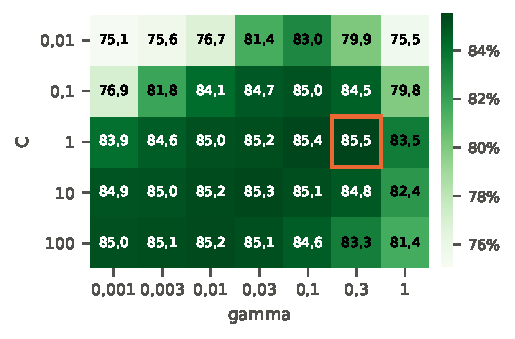
\includegraphics[width=\textwidth]{figures/svm_mapa.pdf}
\caption{Acurácia de validação cruzada (5 partes, seed 0) da SVM RBF por $C$ e $\gamma$. O quadro marca a melhor combinação.}
\label{fig:sv_mapa}
\end{minipage}\hfill
\begin{minipage}[b]{.42\textwidth}
\centering
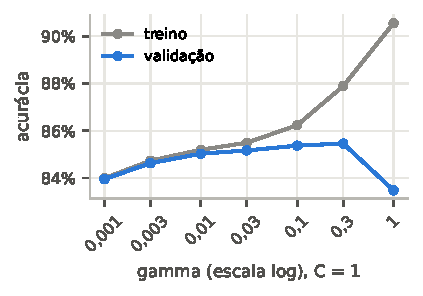
\includegraphics[width=\textwidth]{figures/svm_gamma.pdf}
\caption{Acurácia no treino e na validação por $\gamma$, com $C = 1$ (seed 0).}
\label{fig:sv_gamma}
\end{minipage}
\end{figure}

\textbf{Padronização.} Sem padronização, a SVM RBF cai de \svPadCom\% para \svPadSem\% de acurácia, e o F1 da classe acima de 50 mil, de \svPadFCom\% para \svPadFSem\%; o modelo passa a usar \svPadVetSem{} vetores de suporte (\svPadVetSemPct\% do treino) e leva \svPadTempoSem{} s para treinar, contra \svPadTempoCom{} s (Tabela~\ref{tab:sv_seed0}). O kernel RBF mede a distância entre pessoas somando as diferenças em todos os atributos, e o ganho de capital, que vai até \svGanhoMax, domina essa soma quando não é padronizado~\cite{hsu:03}. A LinearSVC não muda (\svLinPadCom\% e \svLinPadSem\%): o modelo linear dá um peso a cada atributo, e um atributo de escala grande só recebe um peso menor.

\textbf{Tempo por tamanho do treino.} A Figura~\ref{fig:sv_tempo} mede o tempo de treino de cada modelo com 1.000 a \svTreino{} pessoas. Em escala log, a inclinação da reta diz como o tempo cresce. A da SVC é \svInclSVC{} com kernel RBF e \svInclSVCLin{} com kernel linear: dobrar o treino quadruplica o tempo. A da LinearSVC é \svInclLinSVC, tempo proporcional ao treino. Com o treino inteiro, a SVC RBF leva \svTempoSVC{} s, e a LinearSVC, \svTempoLinSVC{} s. A Random Forest é mais lenta que a SVC nos tamanhos pequenos, mas as curvas se cruzam entre 8 e 16 mil pessoas. Pela mesma inclinação, a SVC levaria cerca de 100 s com 100 mil pessoas e horas com um milhão.

\begin{figure}[ht]
\centering
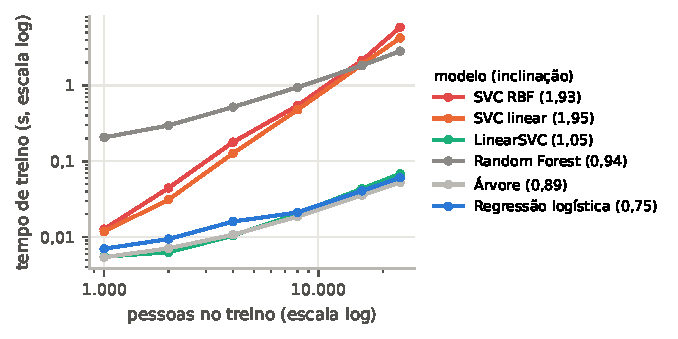
\includegraphics[width=.8\textwidth]{figures/svm_tempo.pdf}
\caption{Tempo de treino (um núcleo, seed 0) por número de pessoas no treino, em escala log nos dois eixos. Entre parênteses, a inclinação da reta ajustada de 4.000 pessoas para cima.}
\label{fig:sv_tempo}
\end{figure}

\subsection{Comparação em 10 seeds}\label{sec:sv_seeds}

A Tabela~\ref{tab:sv_modelos} e a Figura~\ref{fig:sv_acc_auc} reúnem os dez modelos. Nas referências, a regressão logística (\svLogAcc\%) e a árvore ajustada (\svArvAcc\%) ficam a menos de meio ponto uma da outra, e a Random Forest (\svRFAcc\%) fica abaixo da árvore em todas as seeds (\svDifRFArvAcc{} ponto): na configuração padrão, cada árvore cresce até folhas de uma pessoa e decora o ruído dos perfis em conflito. A regra de um corte pergunta, nas 10 seeds, se a pessoa é casada, mas responde ``até 50 mil'' dos dois lados e empata com o piso; sua AUC de \svRegraAuc\% mostra que a pergunta ordena bem as pessoas, e o que falha é o corte. Todos os modelos sem pesos erram cerca de duas vezes mais por falso negativo do que por falso positivo.

\begin{table}[ht]
\centering
\caption{Os dez modelos na base de renda (média $\pm$ desvio em 10 seeds; FP e FN: falsos positivos e negativos em \svTeste{} pessoas de teste, \svPositivosTeste{} delas acima de 50 mil). Tempos: mediana das 10 seeds, num único núcleo; treino do modelo final e previsão do teste inteiro.}
\label{tab:sv_modelos}
\footnotesize
\setlength{\tabcolsep}{3.5pt}
\begin{tabular}{lcccccccc}
\toprule
Modelo & Acurácia (\%) & \shortstack{F1 macro\\(\%)} & \shortstack{F1 $>$50K\\(\%)} & AUC (\%) & FP & FN & \shortstack{Treino\\(s)} & \shortstack{Previsão\\(ms)} \\
\midrule
Classe majoritária & 75,1 $\pm$ 0,0 & 42,9 & 0,0 & 50,0 & 0 & 1.501 & 0,01 & 4,3 \\
Regra de um corte & 75,1 $\pm$ 0,0 & 42,9 & 0,0 & 75,6 & 0 & 1.501 & 0,02 & 4,8 \\
Regressão logística & 84,8 $\pm$ 0,3 & 78,3 & 66,5 & 90,2 & 325 & 592 & 0,06 & 4,5 \\
Árvore de decisão & 85,2 $\pm$ 0,4 & 78,4 & 66,4 & 90,0 & 277 & 617 & 0,06 & 5,1 \\
Random Forest & 84,3 $\pm$ 0,4 & 78,1 & 66,5 & 89,1 & 391 & 559 & 2,8 & 180 \\
\midrule
SVM linear & 84,8 $\pm$ 0,3 & 78,2 & 66,2 & 90,2 & 311 & 604 & 0,05 & 4,5 \\
SVM RBF & 85,4 $\pm$ 0,4 & 79,0 & 67,5 & 88,9 & 294 & 587 & 5,7 & 2016 \\
SVM polinomial & 85,2 $\pm$ 0,4 & 78,7 & 66,9 & 90,2 & 298 & 596 & 3,6 & 488 \\
SVM RBF com pesos & 80,9 $\pm$ 0,3 & 77,6 & 69,0 & 89,8 & 929 & 221 & 6,3 & 2283 \\
Rede neural (MLP) & 85,2 $\pm$ 0,6 & 79,4 & 68,4 & 90,8 & 362 & 533 & 1,0 & 5,6 \\
\bottomrule
\end{tabular}

\end{table}

\begin{figure}[ht]
\centering
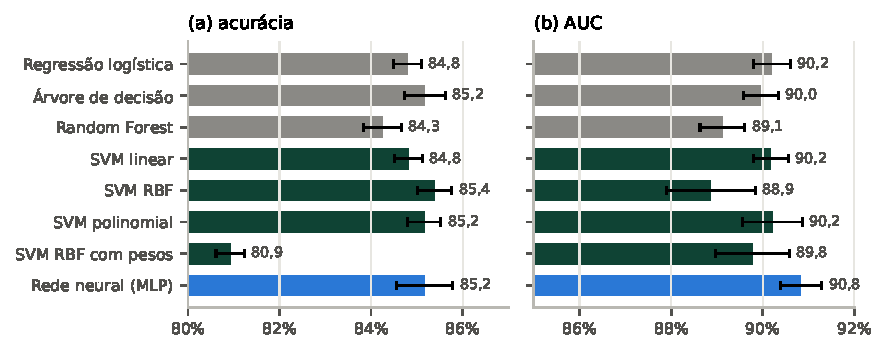
\includegraphics[width=\textwidth]{figures/svm_acc_auc.pdf}
\caption{(a) Acurácia e (b) AUC no teste, média e desvio de 10 seeds. Os eixos começam em 80\% e 85\%. Em verde-escuro, as SVMs.}
\label{fig:sv_acc_auc}
\end{figure}

\textbf{A SVM.} A SVM RBF tem a melhor acurácia, \svRBFAcc~$\pm$~\svRBFSd\%, e o melhor F1 macro entre as SVMs (\svRBFFum\%). Comparando seed a seed, supera a SVM linear em \svSeedsRBFLinAcc{} das 10 seeds (\svDifRBFLinAcc{} ponto) e a Random Forest em \svSeedsRBFRFAcc{} (\svDifRBFRFAcc), mas contra a árvore ajustada fica à frente em só \svSeedsRBFArvAcc{} (\svDifRBFArvAcc{} ponto, menos que o desvio entre seeds): é um empate (teste de Wilcoxon pareado, $p = \svPRBFArvAcc$; contra a SVM linear, $p = \svPRBFLinAcc$, o menor valor possível com 10 seeds). As 10 divisões compartilham os mesmos dados, então os valores de $p$ são otimistas e servem só para separar empate de diferença. A SVM polinomial, de grau 2 em quase todas as seeds, fica entre as duas (\svPoliAcc\%). A SVM linear e a regressão logística são, na prática, o mesmo modelo: \svDifLinLogAcc{} ponto de diferença. A fronteira curva rende, portanto, menos de um ponto sobre a reta, longe do teto de \svTeto\%. A busca foi estável: a SVM RBF escolheu $C = 1$ em \svRBFCUmSeeds{} seeds e a linear, $C = \svLinC$ em \svLinCSeeds{} (Tabela~\ref{tab:sv_grades}).

\textbf{Acurácia contra AUC.} Na AUC a ordem se inverte: a SVM RBF tem \svRBFAuc\%, abaixo da SVM linear e da polinomial (\svLinAuc\% e \svPoliAuc\%), e perde para a linear em todas as seeds (\svDifRBFLinAuc{} ponto). A causa é o critério da busca. A acurácia só olha de que lado da fronteira cada pessoa cai; a AUC olha a ordem das notas. Guiada pela acurácia, a busca prefere $\gamma$ alto, que ajusta bem a fronteira; mas com $\gamma$ alto cada vetor de suporte só influencia a sua vizinhança, e longe deles a nota de quase todos se aproxima do mesmo valor, o que desfaz a ordem entre as pessoas longe da fronteira. Nas \svGTresSeeds{} seeds em que a busca escolheu $\gamma = 0{,}3$, a AUC foi \svGTresAuc\%; nas \svGUmSeeds{} com $\gamma = 0{,}1$, \svGUmAuc\%. E a acurácia no teste nem foi maior com $\gamma = 0{,}3$ (\svGTresAcc\% contra \svGUmAcc\%): a preferência veio de décimos na validação que não se repetiram no teste. Para ordenar pessoas por chance de renda alta, a busca deveria usar a AUC como critério.

\textbf{Pesos por classe.} Com os mesmos $C$ e $\gamma$, os pesos por classe reduzem os falsos negativos de \svRBFFN{} para \svPesosFN: o modelo passa a encontrar \svRecallPesos\% das pessoas de renda alta, contra \svRecallRBF\%. Em troca, os falsos positivos sobem de \svRBFFP{} para \svPesosFP, e a acurácia cai para \svPesosAcc\%. O F1 da classe acima de 50 mil é o maior de todos (\svPesosFpos\%). Qual versão usar depende do custo de cada erro.

\textbf{A rede neural.} A rede chega a \svRedeAcc~$\pm$~\svRedeSd\%, com o melhor F1 macro (\svRedeFum\%) e a melhor AUC (\svRedeAuc\%) dos dez modelos. Na acurácia, a rede supera a SVM RBF em só \svSeedsRedeRBFAcc{} das 10 seeds (\svDifRedeRBFAcc{} ponto); no F1 macro, em \svSeedsRedeRBFFum{} (\svDifRedeRBFFum), um empate; na AUC, em todas (\svDifRedeRBFAuc{} pontos, $p = \svPRedeRBFAuc$; na acurácia, $p = \svPRedeRBFAcc$, e no F1 macro, $p = \svPRedeRBFFum$), e também supera todos os outros modelos na AUC em todas as seeds. A rede é treinada para estimar probabilidades, e suas notas ordenam bem as pessoas em toda a faixa; a SVM só aprende o lado da fronteira. Em troca, varia mais entre seeds: a busca escolheu \svRedeComb{} combinações diferentes em 10 seeds, e a parada antecipada interrompeu o treino entre \svRedeEpMin{} e \svRedeEpMax{} épocas.

\textbf{Tempo.} A SVM com kernel é cara duas vezes. O treino final da SVM RBF leva \svRBFTreino{} s, contra \svLinTreino{} s da SVM linear e \svRedeTreino{} s da rede, e a busca leva \svRBFBusca{} min por seed, contra \svRedeBusca{} min da rede; nas 10 seeds, \svBuscaTotalRBF{} minutos só na busca da SVM RBF. Prever o teste leva \svRBFPrevS{} s, cerca de \svRazaoPrevRBFLin{} vezes a SVM linear e \svRazaoPrevRBFRede{} vezes a rede, porque cada pessoa é comparada com os vetores de suporte (\svRBFVet{}, em média), enquanto a SVM linear e a rede só multiplicam a pessoa por pesos fixos.
